\section{Spectrograms}
The code, that has been used in order to investigate music and female speech signal, is the following:
\begin{lstlisting}
window_length = 0.03; %in ms
num_cepstral  = 13;

[mfccs_f,spectgram_f,f_f,t_f]       = GetSpeechFeatures(y_female,...
                                fs_female,window_length,num_cepstral);
[mfccs_mu,spectgram_mu,f_mu,t_mu]   = GetSpeechFeatures(y_music,...
                                fs_music,window_length,num_cepstral);
[mfccs_ma,spectgram_ma,f_ma,t_ma]   = GetSpeechFeatures(y_male,...
                                fs_male,window_length,num_cepstral);


figure(2)
imagesc(t_f,f_f,log10(spectgram_f)); colormap jet
xlabel('Time in seconds'); ylabel('Frequency in Hz'); title('Female speech');
annotation('textarrow',[0.2 0.25],[0.85 0.9],'String','Voiced'); 
annotation('textarrow',[0.15 0.2],[0.65 0.7],'String','Unvoiced');
figure(3)
imagesc(t_mu,f_mu,log10(spectgram_mu)); colormap jet
xlabel('Time in seconds'); ylabel('Frequency in Hz'); title('Music signal');
annotation('textarrow',[0.2 0.25],[0.83 0.88],'String','Harmonics');
\end{lstlisting}

The results are shown in figure \ref{fig:spec_female_music}. Within the music signal, the harmonics are clearly visible as well as the fact, that the fundamental frequency is changing over time. The same characteristics as in the music signal can be found for voiced sounds within the female speech and is marked by an arrow. The spoken sentence is \textit{I shot an arrow into the air} - the first part of shot, namely \textit{sh}, is unvoiced (feel the larynxgeal prominence). This unvoiced sound occurs after approximately $0.1$ seconds and lasts for nearly $0.15$ seconds and are characterised by a broad spread over the frequency range. Two other occurrences at $0.45$ (the \textit{t} within sho\textbf{t}) and $1.25$ (the \textit{t} within in\textbf{t}o) the seconds are unvoiced. As already discussed, this is also visible within the time domain signal.


\begin{figure}[h]
\centering
\begin{minipage}{.5\textwidth}
  \centering
  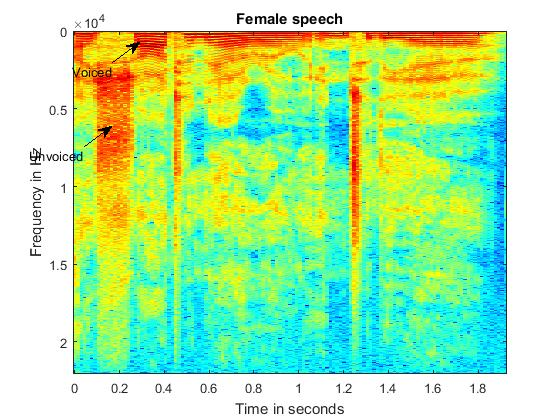
\includegraphics[width=1\linewidth]{./images/spectrogram_female.jpg}
\end{minipage}%
\begin{minipage}{.5\textwidth}
  \centering
  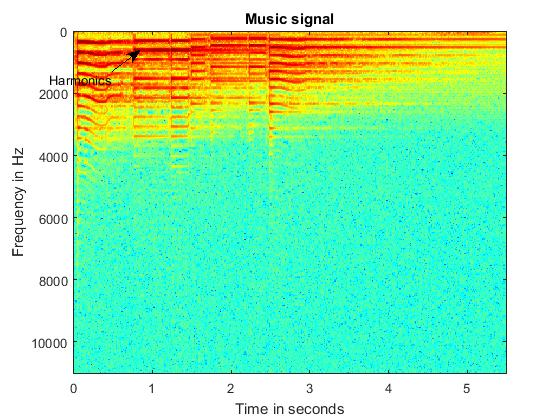
\includegraphics[width=1\linewidth]{./images/spectrogram_music.jpg}
\end{minipage}
 \caption{Spectrogram of femal speech (on the left) and spectrogram of music signal (on the right)}
 \label{fig:spec_female_music}	
\end{figure}
